\chapter{Neutrino oscillations: theoretical background and current status}
\label{chap:theory}

%%%%%%%%%%%%%%%%%%%%%%%%%%%%%%%%%%%%%%%%%%%%%%%%%%%%%%%%%%%%%%%%%%%%%%%%%%%%%%%%%%%%%%%%%%%%%%%%%%
%                                              PLAN                                              %
%%%%%%%%%%%%%%%%%%%%%%%%%%%%%%%%%%%%%%%%%%%%%%%%%%%%%%%%%%%%%%%%%%%%%%%%%%%%%%%%%%%%%%%%%%%%%%%%%%
\begin{comment}
Welcome to neutrino physics, it all began at the beggining of the century with Wolfgang puali etc
etc... Lots of postulating from various people and some really cool experiments with lots of
exciting details later, it was found that there was a neutrino corresponding to each of the
leptons, electon, muon and tau. In the original standard model these are expected to be massless,
charge-0, spin 1/2 particles that are very very waekly interacting with tiny cross sections,
making them an increadibly difficult challenge for experimentalists in the years to come.

It was then noticed by a succesion of different experiments that a few different things did not
add up, the number of neutrinos seen with the expected flavour was wrong. Lots of people then
invested loads of time into tyring to figure this out and it was finally found by SNO which used
channels sensative to the three flavours in different ways, that some neutrinos had turned into
other neutrino flavours, shock horror.

This is explained by supposing that the neutrino flavour states (the ones that interact with the
weak force) are infact a superposition of neutrino mass states. The mixing between these two basis
is described by the PMNS matrix, which contains 3 mixing angles and a phase. An additional two
phases are included if the particles are majorana. What this means is that as the energy states
porpogate through matter differently, he superposition of them leads to neutrino oscillations as
the probability of detecting a certain flavour state changes as the neutrino travels.

The actual oscillation probability derivation is quite complex, and is affected by the matter
through which it travels due to matter having lots of electrons in it. But it generally leads to
sinosoidal probabilities with a phase dependent on the neutrino mass splitting and L/E and an
amplitude dependent on the mixing angles. The single phase, also governs if this oscillation
probability is different between neutrinos and anti-neutrinos and it hence known as the CP
violating phase.

So far we have been able to measure all the phases but we still don't know what delta-cp is, the
octant of theta23 or the mass hierarchy which is the ordering of the masses of the nuutrinos as we
only really measure the mass-spllittings. Splitting the PMNS matrix into the three common areas,
atmospheric, solar and reactor and investigating these three classic experimantal measuring
regions allows us to make conclusions about different parameters and gives us sensitivity to
different neutrino oscillation paramters.

Current experiments such as Nova and T2K are looking at delta-cp and the hierarchy, but it is
likely that we will need ther VERY VERY expensive DUNE experiment to finally figure things out. As
neutrinos very rarely interact it is always a size game with experiments, as all you really are
playing is a counting game. The larger the detection volume, the more nuutrinos you can detect and
as long as you energy resolution is good enough to resolve the oscillations in you particular L/E
regime you have a better experiment than everyone else. VOLUME VOLUME VOLUME, CHEAP CHEAP CHEAP!!!

INTRODUCTION
- Just a brief outline of what I am going to talk about in the theory chapter
- Tell them what you are going to tell them

THE HISTORY OF NEUTRINOS
- How where neutrinos theorised and then discovered
- What where the big problems that led to neutrino oscillations being suggested and then
discovered?

THE THEORY OF NEUTRINO OSCILLATION
- Describe basic neutrino oscillation theory
- derivation of probability in vacuum
- derivation of probability in matter

NEUTRINO INTERACTIONS
- Feynman diagrams of all the main interaction types
- Famous diagrams of cross-section regions for them all
- Descriptions of which types are easy to detect, what are the main NC backgrounds usually etc...

CURRENT EXPERIMENTAL STATUS AND THE FUTURE
- What is the status of each of the three neutrino regimes?
- What are the open questions
- What future experiments could help solve these problems
- CHIPS CHIPS CHIPS
\end{comment}

%%%%%%%%%%%%%%%%%%%%%%%%%%%%%%%%%%%%%%%%%%%%%%%%%%%%%%%%%%%%%%%%%%%%%%%%%%%%%%%%%%%%%%%%%%%%%%%%%%
%                                          INTRODUCTION                                          %
%%%%%%%%%%%%%%%%%%%%%%%%%%%%%%%%%%%%%%%%%%%%%%%%%%%%%%%%%%%%%%%%%%%%%%%%%%%%%%%%%%%%%%%%%%%%%%%%%%
\begin{comment}
-Neutrino physics covers the widest possible range of
-Proposal of a mysterious undetector particle to explain beta decays in the 1930s through to the
resolutions of a 30-year problem with the confirmation of oscillations in the early 2000s and onto
the precision era.
-Neutrino oscillations first discoveed in 1957 when Bruno Pornecorvo proposed a model in which
neutrinos oscilate to antineutrinos and back, similar to the kain. It was actually shown that
neutrinos iscilate from one flavour to another.
-The field of neutrino physics is ever expanding with a new generation of experiments planned for
the coming years.
This chapter aims to provide an introduction to neutrino...
\end{comment}

%%%%%%%%%%%%%%%%%%%%%%%%%%%%%%%%%%%%%%%%%%%%%%%%%%%%%%%%%%%%%%%%%%%%%%%%%%%%%%%%%%%%%%%%%%%%%%%%%%
%                                            HISTORY                                             %
%%%%%%%%%%%%%%%%%%%%%%%%%%%%%%%%%%%%%%%%%%%%%%%%%%%%%%%%%%%%%%%%%%%%%%%%%%%%%%%%%%%%%%%%%%%%%%%%%%
\section{A history of neutrino oscillations}
\label{sec:theory_history}

\subsection{Discovery of the neutrinos} %%%%%%%%%%%%%%%%%%%%%%%%%%%%%%%%%%%%%%%%%%%%%%%%%%%%%%%%%%
\label{sec:theory_history_neutrinos}

In the early 20th century, beta decays were assumed to follow the simple two-body process,
$A \rightarrow B + e$, where nuclei spontaneously emit a single electron. The ejected electron
must have discrete kinetic energy to conserve both energy and angular momentum, defined by the
difference in binding energies between the initial and final nuclei states. However, in 1914,
J. Chadwick instead measured a continuous electron energy spectrum~\cite{chadwick1914}, placing
this theory in doubt.

W. Pauli finally proposed a 'desperate solution' to this paradox in 1930~\cite{pauli1930}. If a
light, neutrally charged, spin $1/2$ particle was also produced in the interaction, the continuous
energy distribution could be explained. Initially, this mysterious new particle was named the
'neutron'. However, to avoid confusion with the heavy baryon of the same name discovered in 1932,
E. Fermi renamed it the 'neutrino' when he formalised beta decay in 1934~\cite{fermi1934}.

The following month, H. Bethe and R. Peierls~\cite{bethe1934} used Fermi's work to estimate the
cross-section of the inverse beta decay process:
\begin{equation} % INVERSE BETA DECAY EQUATION %%%%%%%%%%%%%%%%%%%%%%%%%%%%%%%%%%%%%%%%%%%%%%%%%%%
    \bar{\nu} + p^{+} \rightarrow n + e^{+}.
\end{equation} %%%%%%%%%%%%%%%%%%%%%%%%%%%%%%%%%%%%%%%%%%%%%%%%%%%%%%%%%%%%%%%%%%%%%%%%%%%%%%%%%%%
An upper limit of $10^{-44} cm^2$ was calculated, an incredibly small value, leading them to
declare 'there is no practically possible way of observing the neutrino.' This statement hinted at
the vast difficulties experimentalists would face hunting down and measuring the neutrino in the
years to come.

After an initial tentative identification if 1953, F. Reines and C. Cowan made the first confirmed
observation of the neutrino in 1956~\cite{cowan1956}. Electron antineutrinos produced within the
Savannah River Plan nuclear reactor were detected via the inverse beta decay process outlined
previously. In an underground room of the reactor building, A 'club-sandwich' detector of three
1500 litre liquid scintillator tanks and two 200 litre cadmium doped water target tanks, was
constructed. A total of 330 photomultiplier tubes then measured the two successive characteristic
signals for the interaction allowing for the rejection of the sizeable cosmic ray background.
Firstly, a prompt positron annihilation, followed shortly afterwards by a gamma-ray burst from the
neutron capture by the cadmium.

A second distinct neutrino, the muon neutrino was discovered in 1962 at the Alternating Gradient
Synchrotron (AGS) at Brookhaven~\cite{danby1962}. Protons from the AGS beam incident upon a fixed
target produced charged pions. These would then decay into a beam of muons and neutrinos. After
passing through steel and lead absorbers to remove the muons, neutrino interactions could then be
detected in a series of spark chambers. If only a single neutrino existed, both interactions
\begin{equation} % BROOKHAVEN DECAY EQUATIONS %%%%%%%%%%%%%%%%%%%%%%%%%%%%%%%%%%%%%%%%%%%%%%%%%%%%
    \nu+p^{+}\rightarrow\mu^{+}+n \\
    \nu+p^{+}\rightarrow e^{+}+n
\end{equation} %%%%%%%%%%%%%%%%%%%%%%%%%%%%%%%%%%%%%%%%%%%%%%%%%%%%%%%%%%%%%%%%%%%%%%%%%%%%%%%%%%%
would be expected to occur at the same rate. However, only muons, identified by a single long
track were detected, confirming the existence of the muon neutrino. Not only was this experiment
the first to construct and use an artificial neutrino beam, but it also later went onto win the
1988 Nobel prize for its discovery.

The $Z^{0}$ and $W^{+}$ bosons, the force carriers for the weak force, through which neutrinos
interact, were discovered at the Super Proton Synchrotron at CERN in 1983
~\cite{arnison1983_z,arnison1983_w}. Crucially, as $Z^{0}$ bosons are expected to decay to
neutrinos, measurements made to the decay width can strongly constrain the number of neutrino
flavours. The ALEPH experiment and others at the LEP $e^{+}e^{-}$ collider in the 1990s made
such precise measurements, indicating that the number of light active neutrino flavours to be
$2.984\pm0.008$~\cite{electroweak2006}, see Fig.~\ref{fig:z_resonance}.

\begin{figure} % Z-RESONANCE DIAGRAM %%%%%%%%%%%%%%%%%%%%%%%%%%%%%%%%%%%%%%%%%%%%%%%%%%%%%%%%%%%%%
    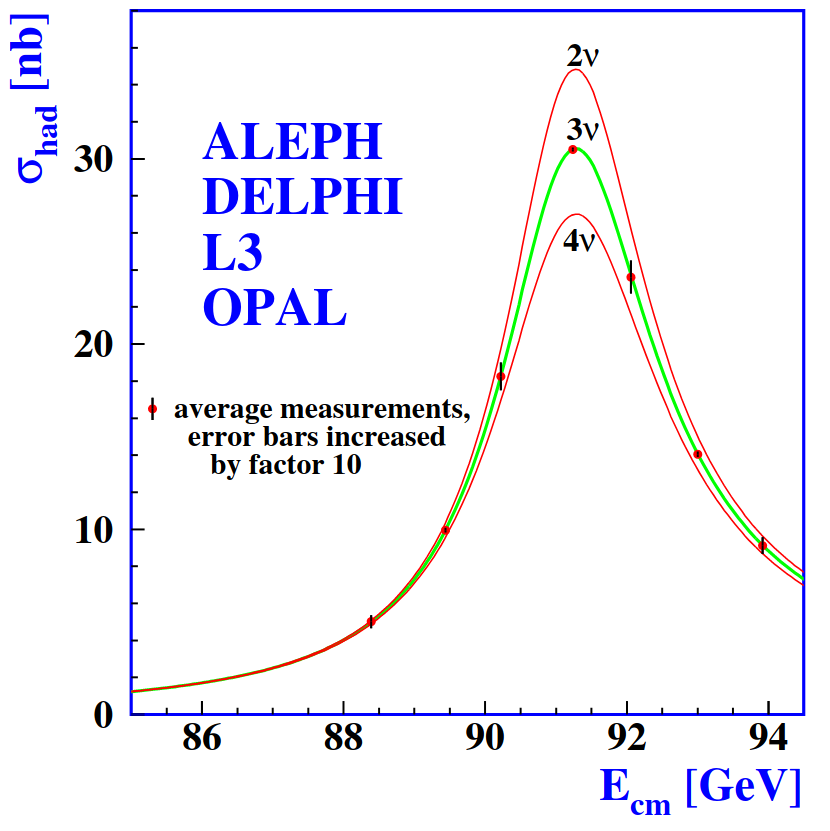
\includegraphics[origin=c,width=0.6\textwidth]{diagrams/3-theory/z_resonance.png}
    \caption[z resonance short]
    {Combined hadron production cross-section measurements around the $Z^{0}$ resonance made by
        experiments at LEP. The curves show the predicted cross-section for two, three, and four
        neutrinos. Note how the data fits the three neutrino hypothesis increadibly well.
        Figure taken from Ref.\cite{electroweak2006}.}
    \label{fig:z_resonance}
\end{figure} %%%%%%%%%%%%%%%%%%%%%%%%%%%%%%%%%%%%%%%%%%%%%%%%%%%%%%%%%%%%%%%%%%%%%%%%%%%%%%%%%%%%%

Combined with the discovery of the tau lepton in 1975~\cite{perl1975}, this suggested that there
was a third tau neutrino. The DONUT experiment at Fermilab finally discovered this particle in
2001~\cite{Kodama2001} using 800\GeV Protons from the Tevatron, completing the trio of neutrinos
we know of today. Any additional neutrinos must either be "sterile"(do not couple to the weak
force) or have a mass greater than $0.5m_{Z}$.

\subsection{Discovery of neutrino oscillations} %%%%%%%%%%%%%%%%%%%%%%%%%%%%%%%%%%%%%%%%%%%%%%%%%%
\label{sec:theory_history_neutrinos}

At the Homestake mine\footnote{The Homestake mine will also be used for the future DUNE experiment
    discussed later} in the 1960s, a large tank, placed 1.5 km underground, was filled with
400000 litres of the dry cleaning fluid, perchloroethylene ($C_{4}Cl_{8}$). Its goal was to
measure the solar electron neutrino flux incident upon the earth via the interaction:
\begin{equation} % HOMESTAKE CHLORINE EQUATION %%%%%%%%%%%%%%%%%%%%%%%%%%%%%%%%%%%%%%%%%%%%%%%%%%%
    {}^{37}Cl+\nu_{e}\rightarrow{}^{37}Ar+e^{-},
\end{equation} %%%%%%%%%%%%%%%%%%%%%%%%%%%%%%%%%%%%%%%%%%%%%%%%%%%%%%%%%%%%%%%%%%%%%%%%%%%%%%%%%%%
allowing the neutrino flux to convert the chlorine contained within the tank to the noble gas
argon. Every few weeks the tank was purged with gaseous helium and via a cooled carbon trap the
amount of argon generated, and indirectly the neutrino flux measured.

After analysis, the number of electron neutrino interactions per ${}^{37}Cl$, per second was found
to be no higher than 3~\cite{davis1968}. Compared to the predictions made by the Standard Solar
Model ranging between 4.4 and 22~\cite{bahcall1968}, this indicated a deficit. Dubbed the
'solar neutrino problem' it was initially believed to be due to an unexplained experimental flaw.
However, other experiments, such as the water Cherenkov Kamiokande II~\cite{hirata1989} and both
the SAGE and GALLEX galium based capture tanks also observed this discrepancy.

A neutrino deficit was also observed indirectly in the atmospheric sector. Neutrinos generated in
the atmosphere by cosmic rays formed a key background to the Kamiokande and IMD experiments, both
designed to measure proton decay. When evaluating the background, they observed a deficit in the
number of muon neutrinos compared to electron neutrinos~\cite{hirata1988, becker1992}. The
successor to the Kamiokande experiment Super-Kamiokande also measured the same deficit
~\cite{kajita1999}.

The phenomenon of neutrino oscillations was put forward as a solution to this problem. If
neutrinos could change flavour as they propagated, it would be expected to find deficits of a
particular flavour as they oscillated to another flavour. The SNO experiment finally confirmed
this in 2001~\cite{ahmad2002}.

Consisting of a 1kton tank of deuterium (heavy water), equiped with 9500 photomultiplier tubes the
SNO experiment was able to measure the light from three seperate solar neutrino interaction
channels:
\begin{align} % SNO INTERACTIONS EQUATIONS %%%%%%%%%%%%%%%%%%%%%%%%%%%%%%%%%%%%%%%%%%%%%%%%%%%%%%%
    \nu_{i}+e^{-} & \rightarrow \nu_{i}+e^{-} \\
    \nu_{i}+d     & \rightarrow p+n+\nu_{i}   \\
    \nu_{e}+d     & \rightarrow p+p+e^{-}
\end{align} %%%%%%%%%%%%%%%%%%%%%%%%%%%%%%%%%%%%%%%%%%%%%%%%%%%%%%%%%%%%%%%%%%%%%%%%%%%%%%%%%%%%%%
where $d$ is the deuterium nucleus. The first and second channels were sensitive to all three
neutrino flavours, but importantly only electron neutrinos could interact via the third channel.
By comparing the rates between the channels, SNO was able to prove to 5.3 sigma that electron
neutrinos had oscillated to other flavours, while the total solar neutrino flux remained constant.

%%%%%%%%%%%%%%%%%%%%%%%%%%%%%%%%%%%%%%%%%%%%%%%%%%%%%%%%%%%%%%%%%%%%%%%%%%%%%%%%%%%%%%%%%%%%%%%%%%
%                                       OSCILLATION THEORY                                       %
%%%%%%%%%%%%%%%%%%%%%%%%%%%%%%%%%%%%%%%%%%%%%%%%%%%%%%%%%%%%%%%%%%%%%%%%%%%%%%%%%%%%%%%%%%%%%%%%%%
\section{Neutrino oscillation theory}
\label{sec:theory_theory}

\begin{comment}
- B. Pontecorvo first described neutrino oscillation, by nautrino and anti nuetrinos in 1957,
later Maki, Nakagawa and Sakata in 1962 included electon and muon neutrino mixing
- The original standard model had the neutrinos as massless. But given that neutrinos oscillations
have been observed this is now not valid.
- It is possible to modify the standard model to allow for this fact without new physics, but it
is generally considered to be a significant break in the SM.
- Can be explained by the quantum pheneomentum of interferance.
- With the flavour and mass eigenstates not being evuivalent, this mixing is described by the
rotation PMNS matrix, analogous to the CKM mixing describing mixing in the quark sector.
- The energy state propogation is well defined, causing the neutrino flavour to change with time
in an oscillatory fashion. Such that a muon neutrino after travelling a distance can be detected
as a electon of tau neutrino but after another distance be detector as a muon neutrino again.

- The neutrino has no electric charge, virtually no mass, and can travel undetectably for vast
distances.
- How does the standard model allow for neutrino masses?
- Fermi vs majorana mass terms, which one is more likely etc
DIAGRAM: For a given fixed baseline, show the oscillation probability as a function of energy, do
this for the chips location.
- Talk about the full neutrino oscillation equations, but also the simplified ones and then how
they affect the shape of the probability curves.
EQUATION: Basic neutrino oscillation equations
EQUATION: Neutrino oscillations in matter equations
EQUATION: Matter effect equations
- We look at the oscillation structure across a range of energies in our detectors to measure the
oscilaltion parameters.
INFO: How the shape of the neutrino flux at the far detector affects the parameters, reduction
fraction, position of the dip etc... maybe a little diagram

- The changing state of the neutrino flavour as it propogates can be explained by having the
flavour eigenstates through which the neutrinos
couple to the weak force be different from their energy eigenstates for the matter through which
the neutrinos are travelling.
- With the flavour eigenstates being expresses as a superposition of the energy states, neutrino
oscillations arise through interference due tof
the energy states evolving differently with time.
- Free particles travelling in a vacuum can be trated as plane waves $E=\sqrt{p^2+m^2}$ therefore,
the energy eigenstates have a well-defined mass,
this then implies than there must be three mass states for the neutrinos with different quantum
numbers, atleast two must be non-zero.
- To understand neutrinos you need, a flavour basis, an orthonormal energy basis with three energy
esigenstates for the medium, eigenvalues of those energy states,
and a unitary matrix to convert between the basis.
- Using the simplified approximation of treating the neutrino states as plane waves, we can simply
derive the oscilaltion probabilities.
- Main flaw with this assumption is that plane waves are not localised and can not describe the
localised interactions of neutrinos.
- Additionally neutrinos have differing energy and momentum not a common one approximation as c.
- These can be solved when the neutrino states are described as wave packets, but this derivation
is much simpler and gets to the same equally correct result.

- In a vacuum, a unitary mixing matrix describes the mixing of mass states to produce the flavour
states. and vice-versa
- In the case of three neutrino flavours the unitary mixing matrix is called the Pontecorvo, Maki,
Nakata and Sakawa matrix, PMNS.
- Analagous to the CKM (Cabibbo-Kobayashi-Maskawa) matrix.
- $\mathrm{U}_{\mathrm{PMNS}}$ is a unitary, complex, $3\times3$ matrix. Which can be desribed by
$n^{2}$ parameters, with $n(n-1)/2$ angles
and $n(n+1)/2$ phases, 3 mixing angles $\theta_{12}$, $\theta_{23}$ and $\theta_{13}$ and six
complex phases.
- Some of these phases can be removed as it desribes the mixing between particle fields, hence no
physical processes are affected.
- They are absorbed into the neutrino fields.
- If Dirac particles then just one pahse is left $\delta_{CP}$ if Majorana you get an additional
two phases $\alpha_{12}$ and $\alpha_{31}$ which lie on the diagonal and hence have no effect on
neutrino oscillations.
\end{comment}

\begin{align} % NEUTRINO MIXING EQUATION %%%%%%%%%%%%%%%%%%%%%%%%%%%%%%%%%%%%%%%%%%%%%%%%%%%%%%%%%
    \ket{\nu_{\alpha}} & = \sum_{k}U_{\alpha k} \ket{\nu_{k}}          \\
    \ket{\nu_{k}}      & = \sum_{k}U_{\alpha k}^{*} \ket{\nu_{\alpha}}
\end{align} %%%%%%%%%%%%%%%%%%%%%%%%%%%%%%%%%%%%%%%%%%%%%%%%%%%%%%%%%%%%%%%%%%%%%%%%%%%%%%%%%%%%%%

\begin{gather} % PMNS MATRIX SIMPLE %%%%%%%%%%%%%%%%%%%%%%%%%%%%%%%%%%%%%%%%%%%%%%%%%%%%%%%%%%%%%%
    \begin{pmatrix}
        \ket{\nu_{e}}   \\
        \ket{\nu_{\mu}} \\
        \ket{\nu_{\tau}}
    \end{pmatrix}
    =
    \begin{pmatrix}
        U_{e1}     & U_{e2}     & U_{e3}     \\
        U_{\mu 1}  & U_{\mu 2}  & U_{\mu 3}  \\
        U_{\tau 1} & U_{\tau 2} & U_{\tau 3}
    \end{pmatrix}
    \begin{pmatrix}
        \ket{\nu_{1}} \\
        \ket{\nu_{2}} \\
        \ket{\nu_{3}}
    \end{pmatrix}
\end{gather} %%%%%%%%%%%%%%%%%%%%%%%%%%%%%%%%%%%%%%%%%%%%%%%%%%%%%%%%%%%%%%%%%%%%%%%%%%%%%%%%%%%%%

\begin{align} % DIRAC PMNS MATRIX FULL %%%%%%%%%%%%%%%%%%%%%%%%%%%%%%%%%%%%%%%%%%%%%%%%%%%%%%%%%%%
    \mathrm{U}_{\mathrm{PMNS}} & =
    \begin{pmatrix}
        1 & 0       & 0      \\
        0 & c_{23}  & s_{23} \\
        0 & -s_{23} & c_{23}
    \end{pmatrix}
    \begin{pmatrix}
        c_{13}                   & 0 & s_{13}e^{-i\delta_{CP}} \\
        0                        & 1 & 0                       \\
        -s_{13}e^{-i\delta_{CP}} & 0 & c_{13}
    \end{pmatrix}
    \begin{pmatrix}
        c_{12}  & s_{12} & 0 \\
        -s_{12} & c_{12} & 0 \\
        0       & 0      & 1
    \end{pmatrix}
    \\
                               & =
    \begin{pmatrix}
        c_{12}c_{13}
         & s_{12}c_{13}
         & s_{13}e^{-i\delta_{CP}}                          \\
        -s_{12}c_{23}-c_{12}s_{23}s_{13}e^{i\delta_{CP}}
         & c_{12}c_{23}-s_{12}s_{23}s_{13}e^{i\delta_{CP}}
         & s_{23}c_{13}                                     \\
        s_{12}s_{23}-c_{12}c_{23}s_{13}e^{i\delta_{CP}}
         & -c_{12}s_{23}-s_{12}c_{23}s_{13}e^{i\delta_{CP}}
         & c_{23}c_{13}
    \end{pmatrix}
\end{align} %%%%%%%%%%%%%%%%%%%%%%%%%%%%%%%%%%%%%%%%%%%%%%%%%%%%%%%%%%%%%%%%%%%%%%%%%%%%%%%%%%%%%%


with $s_{ij}=\sin \theta_{ij}$ and $c_{ij}=\cos \theta_{ij}$

\begin{equation} % PLANE WAVE EQUATION %%%%%%%%%%%%%%%%%%%%%%%%%%%%%%%%%%%%%%%%%%%%%%%%%%%%%%%%%%%
    \psi(x,t=0)=\sum_{i=1}^{3}U_{\alpha k}e^{ip_{\alpha}x}
\end{equation} %%%%%%%%%%%%%%%%%%%%%%%%%%%%%%%%%%%%%%%%%%%%%%%%%%%%%%%%%%%%%%%%%%%%%%%%%%%%%%%%%%%

%%%%%%%%%%%%%%%%%%%%%%%%%%%%%%%%%%%%%%%%%%%%%%%%%%%%%%%%%%%%%%%%%%%%%%%%%%%%%%%%%%%%%%%%%%%%%%%%%%
%                                     NEUTRINO INTERACTIONS                                      %
%%%%%%%%%%%%%%%%%%%%%%%%%%%%%%%%%%%%%%%%%%%%%%%%%%%%%%%%%%%%%%%%%%%%%%%%%%%%%%%%%%%%%%%%%%%%%%%%%%
\section{Neutrino interactions}
\label{sec:theory_interactions}

\begin{figure} % CROSS-SECTION DIAGRAM %%%%%%%%%%%%%%%%%%%%%%%%%%%%%%%%%%%%%%%%%%%%%%%%%%%%%%%%%%%
    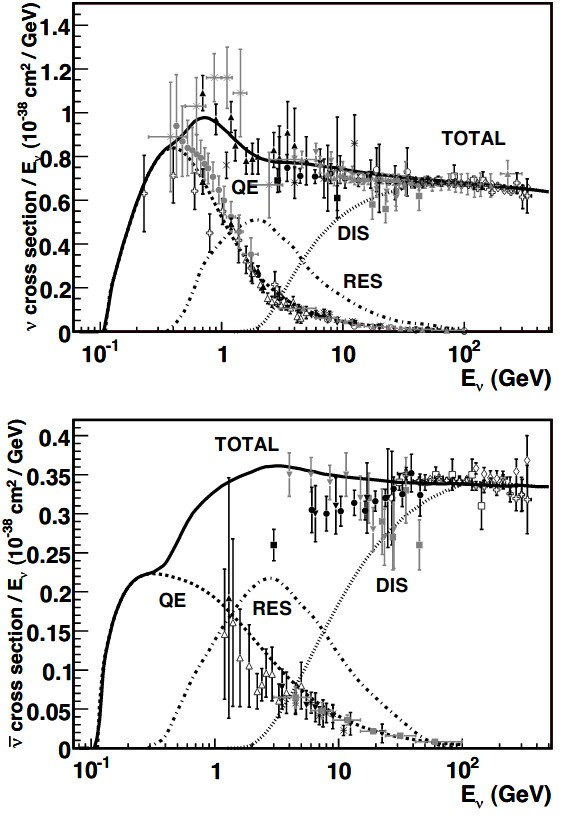
\includegraphics[origin=c,width=0.6\textwidth]{diagrams/3-theory/cross_sections.png}
    \caption[cross sections short]
    {Figure taken from Ref.\cite{formaggio2012}.}
    \label{fig:cross_sections}
\end{figure} %%%%%%%%%%%%%%%%%%%%%%%%%%%%%%%%%%%%%%%%%%%%%%%%%%%%%%%%%%%%%%%%%%%%%%%%%%%%%%%%%%%%%

\begin{figure} % TAU CROSS-SECTION DIAGRAM %%%%%%%%%%%%%%%%%%%%%%%%%%%%%%%%%%%%%%%%%%%%%%%%%%%%%%%
    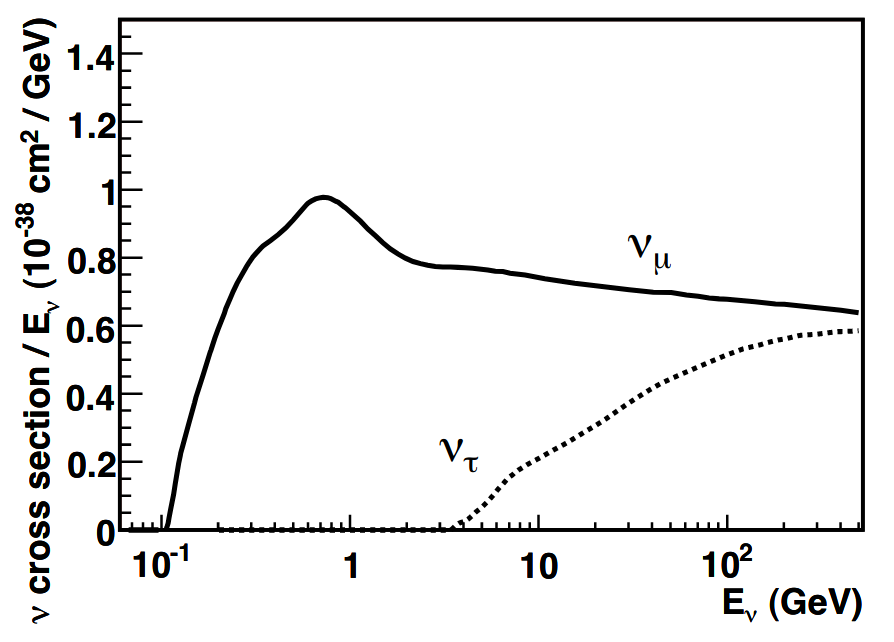
\includegraphics[origin=c,width=0.6\textwidth]{diagrams/3-theory/tau_comparison.png}
    \caption[tau comparison short]
    {Figure taken from Ref.\cite{formaggio2012}.}
    \label{fig:tau_comparison}
\end{figure} %%%%%%%%%%%%%%%%%%%%%%%%%%%%%%%%%%%%%%%%%%%%%%%%%%%%%%%%%%%%%%%%%%%%%%%%%%%%%%%%%%%%%

\begin{figure} % FEYNMAN INTERACTION TYPE DIAGRAMS %%%%%%%%%%%%%%%%%%%%%%%%%%%%%%%%%%%%%%%%%%%%%%%
    \feynmandiagram[horizontal=a to b] {
    i1 [particle=\(e^{-}\)] -- [fermion] a -- [fermion] i2 [particle=\(e^{+}\)],
    a -- [photon, edge label=\(\gamma\), momentum'=\(k\)] b,
    f1 [particle=\(\mu^{+}\)] -- [fermion] b -- [fermion] f2 [particle=\(\mu^{-}\)],
    };
    \feynmandiagram[horizontal=a to b] {
    i1 [particle=\(e^{-}\)] -- [fermion] a -- [fermion] i2 [particle=\(e^{+}\)],
    a -- [photon, edge label=\(\gamma\), momentum'=\(k\)] b,
    f1 [particle=\(\mu^{+}\)] -- [fermion] b -- [fermion] f2 [particle=\(\mu^{-}\)],
    };
\end{figure} %%%%%%%%%%%%%%%%%%%%%%%%%%%%%%%%%%%%%%%%%%%%%%%%%%%%%%%%%%%%%%%%%%%%%%%%%%%%%%%%%%%%%

\begin{comment}
- From eV to EeV: Neutrino Cross-Sections Across Energy Scales
- Neutrino originally postulated by Wolfgang Pauli in 1930, and has played a prominent role in
understanding of nuclear and particle physics.
- The revalation that neutrinos can no longer be massless is perhaps the first significant
alteration to the standard model.
- A nice plot of neutrino energy regimes from Big Bang through accelerator to Extra-galactic vs
their cross-sections. I could definitely use this and cite it to the paper
- Contains a good description of fundamental electroweak scattering if we need a reference for
that (page 4->)
- First anumu + e- => anumu + e- scattering made by CERN bubble cchamber experiment Gargamelle
- This and DIS NC observations confirmed the weak neutral currents and helped solidify the
standard model.
- Maybe include a bubble chamber image of the first candidate neutrino interaction.
- At intermediate energy scales (CHIPS range) interactions fall into three main catageories.
Elastic and quasi-elastic scattering, resonance production and DIS.
- Include an actual data cross-section plot for both CC and NC showing contributions from
different experiments
- Show the tau-neutrino cross section compared to the muon/electron in our energy range to show it
doesn't matter. All the interactions and arguments that go along with them are the same for
nuel/numu as with nutau, except for one key difference; the energy threshold. The nutau
interaction CC cross section is severely altered because of the large tau lepton mass. Then
show the plot.
- Bellow 2Gev it's mainly quasi-elastic with the neutrino scattering of the entire nucelon, rather
than its consituent partons.
- Modern experiments MiniBooNE and NOMAD see higher absolute cross-sections than expected. It is
currently believed that nucelear effects beyond the impulse approximation are desponsible for the
discrepancy. Such as nucleon-nucleon correlations and two-body exchange currents must be included
to get it righ. THIS IS MEC!
- NC QEL lots of people call NC Elastic Scattering, the ratio of NC Elastic/CC QE is ~0.11 from
measurements by a few experiments.
- Single pion production is when the neutrino excites the struck nucleon producing a baryon
resonance, which then quickly decays most often into a nucleon and a single pion final state.
There are seven possible single pion channels, 3CC and 4NC, which we see from the GENIE events.
- Show all the interaction equations for these %νμp→μ−pπ+ etc...
- NC pi-zero production is often the largest numu-induced backgrond in experiments searching for
numu->nuel oscillations. And CC pi production can present a non-negligable complication in the
determination of neutrino energy in experiments. Therefore measuring and modelling nuclear effects
in pion production has become paramount.
- These resonances can also decay into photons with a small branchng fraction, yes, but, like NC
pi-zero production they still pose a non-negliable source of background to the CHIPS main search.
- Neutrinos can also coherently produce single pion final state. In this case the neutrino
coherently scatters from the entire nucleus transferring negligable energy to the target. Hence,
you produce a ditinctly forward-scattered pion with no nuclear recoil. This process is relatively
small however.
- The resonances can also decay to multi-pion final state, along with DIS this contributes a
copious source of multi-pion final states. However, due to the inherant complexity of
reconstructing multiple pion final states, not many experiments look at these cross-sections.
- You can also get kaon production but they have small cross-sections due to the kain mass and
because kaon channels are not enhanced by any dominant resonance.
- You then get DIS where the neutrino scatters of a quark in the nucleon via the exchange of a
virtual W or Z boson producing a lepton and a hadronic system in the final state.
- To isolate DOS events experiments typically apply kinematic cuts to remove QE scattering and
resonance-mediated contributions from their data.
\end{comment}

%%%%%%%%%%%%%%%%%%%%%%%%%%%%%%%%%%%%%%%%%%%%%%%%%%%%%%%%%%%%%%%%%%%%%%%%%%%%%%%%%%%%%%%%%%%%%%%%%%
%                                 CURRENT STATUS AND THE FUTURE                                  %
%%%%%%%%%%%%%%%%%%%%%%%%%%%%%%%%%%%%%%%%%%%%%%%%%%%%%%%%%%%%%%%%%%%%%%%%%%%%%%%%%%%%%%%%%%%%%%%%%%
\section{Current status and the future}
\label{sec:theory_status}

\begin{comment}
- Over that last 20 years neutrino oscillations have become well-established and we are now moving
into the precision measurement era.
- DUNE is a next-generation neutrino oscillation experiment with a primary scientific goal of
observation of CP-violation in the neutrino sector.
- In DUNE a muon neutrino(anti-neutrino) beam will be produced by the Long-Baseline Neutrino
Facility (LBNF)
- There will be a near detector at Fermilab before the neutrinos travel the 1285km to the Sanford
Underground Research Facility (SURF) in South Dakota.
- The far detector will consist of four 10kt (fiducial) liquid argon time projections chamber
(LArTPC) detectors.
- Neutrino oscillation probabilities can then be infered by comparisons of the observed neutrino
spectra and the near and far detectors.
- Recent obsevation of a large theta13 have focuseed the next genetation of long baseline
experiments towards the mass hierarchy, octant of theta23 and measureing delta-CP
- Nova and T2k will not be able to measure the remaining unknows (check this)
- Dune will hopefully solve these problems but will be increadibly expensive

- Symmetries under charge-conjugation and parity inversion are both macimally violated by the
waek interaction.
- Their combined operation has been shown to be violated, to a small degress, by quark mixing
processes.
- If sin(delta-cp) is non zero then vacuum oscillation properties of nu and anti nu will be
different.
- DUNE (I assume CHIPS) is sensative to four oscillation paramters, delta31, theta23, theta13
and delta-cp.
- These can be measured using four data sample, two for neutrino and two for antineutrinos.
- These sample are produced by "Forward Horn current" FHC and "Reverse Horn current" RHC,
producing predominetetly neutrinos and anti-neutrinos respectively.
- Dissapearence channels sensitive to %abs(delta31^2), and sin^2(2theta23).
- Apperence channels sensitive to all four parameters including sign of %delta32^2.
- The "signal" in all cases are CC interactions, therefore selection of nuel, anuel, numu and
anumu CC is the goal.
- Main background in CC numu selections are NC with charged pions.
- Main background in CC nuel selections is pi-zero NC, which can mimic the chracteristic EM
shower, due to its near certain decay into two photons.
- You get a small number of nuel intrinsic to the beam, they are just a background as they are
indistinguishabe from the nuel appreaence neutrinos.
- Once you have collected samples in all four cases, a fit is performed to the reconstructed
neutrino energy distributions to extract the four neutrino oscillation parameters.
- How is the absolute nuetrino energy constrained\dots
- KATRIN upper limit of 1.1eV (90percent confidence level) on the absolute mass of the neutrinos.
KATRIN mass in in Ref.~\cite{aker2019}
\end{comment}